\chapter{Dvojrozmerné polia}
\label{sect:2dpolia}

Po troch vysvetľujúcich kapitolách poďme naspäť k programovaniu. 
Chceme riešiť takúto úlohu: na vstupe sú dve čísla $r$ a $s$ a potom 
tabuľka čísel s $r$ riadkami a $s$ stĺpcami. Úlohou je napísať program, ktorý
tabuľku otočí takto: 

\begin{column}{0.45}
\vbox{
Vstup:\\
\vb{
3 4 \\[1ex]
\begin{tabular}{@{\hspace*{0pt}}cccc}
0&1&2&3\\
  4&5&6&7\\
  8&9&10&11
\end{tabular}
}
}
\end{column}
\hfill
\begin{column}{0.45}
\vbox{
Výstup:\\
\vb{
\begin{tabular}{@{\hspace*{0pt}}ccc}
  0&4&8\\
  1&5&9 \\
  2&6&10\\
  3&7&11
\end{tabular}
}
}
\end{column}


Jeden prístup je prečítať celý vstup do jedného poľa veľkosti $rs$:\\

\vbox{
\begin{lstlisting}[] 
int r, s, i;
cin >> r >> s;
int a[r * s];
for (i = 0; i < r * s; i++) cin >> a[i];
\end{lstlisting}
}

 Fajn, ale ako ho vypísať? Keď si očíslujeme riadky aj stĺpce od 0, tak vidíme,
že číslo v riadku $i$ a stĺpci $j$ bude na pozícii $is+j$:  pred ním je $i$ celých
riadkov po $s$ čísel a ešte $j$ čísel z riadku $i$. Napr. v riadku $2$ a stĺpci $1$ je
číslo $9$:\\


\centerline{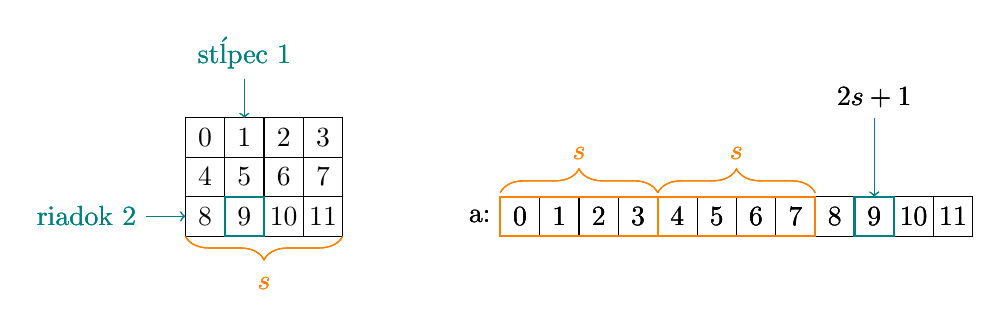
\begin{tikzpicture}[scale=0.5]
  \def\row#1#2#3{%
    \draw[#3] decorate[
       decoration={brace, amplitude=2ex}]{
       (#1,1.1) -- (#1+4,1.1) node [align=center,midway,anchor=south,yshift=2ex] {$#2$}
        };
   \draw[#3,thick] (#1,0) rectangle (#1+4,1);
  }
  \foreach \i in {0,...,2} {
    \foreach \j in {0,...,3} {
       \pgfmathtruncatemacro{\v}{\i*4+\j}
       \draw(\j,-\i) rectangle node[anchor=center] {\vb{\v}}  (\j+1,-\i+1) ;
     }
  \draw[teal, -> ] 
    (-1,-1.5) node[anchor=east]{riadok 2} -- (0,-1.5);
  \draw[teal,->]
  (1.5, 2) node[anchor=south]{stĺpec 1} -- (1.5,1);
  \draw[teal,thick] (1,-2) rectangle (2,-1);
    
  \draw[orange] decorate[
       decoration={brace, amplitude=2ex}]{
       (4,-2) -- (0,-2) node [align=center,midway,anchor=north,shift={(0,-0.4)}] {$s$}
        };
 
  \begin{scope}[shift={(8,-2)}]
    \foreach \x in {0,...,11} {
      \draw (\x,0) rectangle node[anchor=center]{\vb{\x}} (\x+1,1);
    }
    \row0{s}{orange}  
    \row4{s}{orange}  
    \draw[teal,thick] (9,0) rectangle (10,1); 
    \draw[teal, ->] (9.5,3) node[black,anchor=south]{$2s+1$} -- (9.5,1);
    \draw (0,0.5) node[anchor=east] {\vb{a:}};
  \end{scope}

}
\end{tikzpicture}}

Vypisovanie vieme urobiť tak, že v jednom cykle (v premennej \prg!j!)
prechádzame po stĺpcoch a pre každý stĺpec ideme v druhom cykle po všetkých
číslach toho stĺpca a vypíšeme ich:\\

\vbox{
\begin{lstlisting}[] 
for (j = 0; j < s; j++) {
  for (i = 0; i < r; i++)
    cout << a[i * s + j] << " ";
  cout << endl;
}
\end{lstlisting}
}

Aby sa nám takéto výpočty zjednodušili, môžeme použiť dvojrozmerné pole, ktoré
vytvorí tabuľku premenných. Príkaz \prg!int a[3][4];! vyrobí premenné\\\indexItem{Prg}{dvojrozmerné pole}


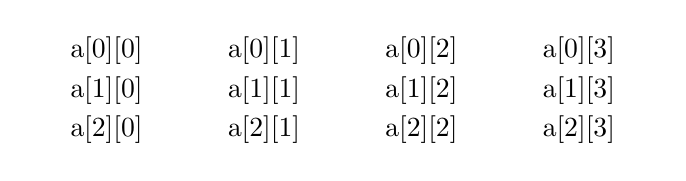
\begin{tikzpicture}[xscale=2,yscale=0.5]
  \foreach \i in {0,...,2}
  \foreach \j in {0,...,3} {
    \draw[draw=none] (\j,-\i) rectangle node [anchor=center]{\vb{a[\i][\j]}} (\j+1,-\i+1);
  }
\end{tikzpicture}

Celý program bude vyzerať takto:\\

\vbox{
\begin{lstlisting}[] 
#include <iostream>
using namespace std;
int main() {
  int r, s, i, j;
  cin >> r >> s;
  int a[r][s];

  for (i = 0; i < r; i++)    // cyklus pre riadky
    for (j = 0; j < s; j++)  // cyklus pre stĺpce
      cin >> a[i][j];

  for (j = 0; j < s; j++) {  // vypíšeme vymenené riadky a stĺpce
    for (i = 0; i < r; i++) 
      cout << a[i][j] << " ";
    cout << endl;
  }
}
\end{lstlisting}
}

\begin{uloha}
  Na vstupe sú čísla $r$, $s$, $d$ a tabuľka čísel s $r$ riadkami a $s$ stĺpcami.
  Napíšte program, ktorý zistí, či sa v tabuľke vyskytuje štvorec $d\times d$
  zo samých núl.
\end{uloha}
